\section{Smart Time Slice Scheduler}
\label{sec:synchronization-approach}

Using \algalpha~ensures an adaptiveness to link quality changes. 
Still, this algorithm does not take into account bad chunk scheduling decisions for end-of-file scenarios as depicted in~\fref{fig:bad-scheduling} (a). 
In this section we introduce the \algslice~algorithm, which takes such end-of-file scenarios into account. 

Key idea of this scheduler is that in order to optimally bundle the throughput performance of each active path we have to optimize the path synchronization. 
Path synchronization means that the traffic should be distributed in a way such that each path finishes downloading its very last chunk at the same time, keeping each path busy and thus reducing unnecessary idle times.
We propose a scheduling algorithm whose goal is to determine an optimal download time span for each chunk. 
Together with the throughput and round-trip-time estimates of each active path we can determine a chunk size for optimal path synchronization.

In the following we introduce our algorithm for two active connections for simplicities sake, but the algorithm can be easily converted to also work with more than two connections.

Let $c_1$ and $c_2$ be the connections established by \mhttp. 
We define $\overline{R}_i$ and $\overline{rtl}_i$ as the estimated throughput and latency (round trip) of $c_i$, and by $s_{i,j}$ we denote the size of the $j$th chunk to be transmitted over $c_i$. 
In~\xref{sec:metrics} we explain in detail how $\overline{R}_i$ and $\overline{rtl}_i$ are estimated.
The task of the scheduler is to determine $s_{i,j}$ upon the completion of the download of the $(j-1)$-th chunk.

%Chunk scheduling means making decisions for the size of each request range $s_{i,j}$ with $j=1,2,3 \cdots, n$ for a connection $c_{i}$. 


%We define $R_i$, $rtt_i$ and $T_{i,j}$ as the estimated throughput and round-trip-time of connection $i$ and the estimated optimal time span of chunk $j$ for connection $i$ repsectively. 
%We use harmonic mean to estimate the trhoughput $R_i$ on every socket read operation. 
%Given a series of bandwidth measurements $\overline{R}_i(t)$, where $t=0,1,2,\cdots, n-1$, the harmonic mean can be calculated with
%(TODO: ref Yung-Chih Paper):
%
%$$R_i = \frac{n+1}{\frac{n}{R_i} + \frac{1}{\overline{R}_i(n+1)}}$$

%The round-trip-time $rtt_i$ is estimated on every received response header with a moving average as described in section~\ref{sec:metrics}. 
%The optimal $j$th chunk size of connection $i$, $s_{i,j}$ is defined as: 

%$$s_{i,j} = R_i \cdot T_{i,j}$$

\begin{figure*}[t]
		\begin{minipage}[t]{0.3\linewidth}
		\begin{center}
                \subfigure[Scheduler $\beta$: For $c_1$ the closest estimated time $\beta_{i,j}$ until another connection finishes downloading its current chunk.]{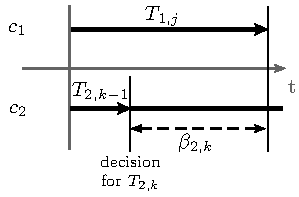
\includegraphics[width=\linewidth]{Figures/scheduler-beta.pdf}}
        \end{center}
        \end{minipage}
~
        \begin{minipage}[t]{0.3\linewidth}
		\begin{center}
                \subfigure[Scheduler Case 1: $c_1$ can download the remaining bytes in the next request while staying within its upper boundary $T_{1,max}$ and before $c_2$ finishes downloading its current chunk.]{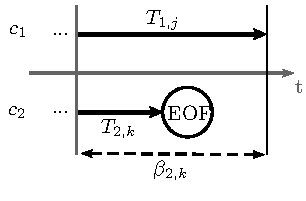
\includegraphics[width=\linewidth]{Figures/scheduler-case-1.pdf}}
        \end{center}
        \end{minipage}
~
        \begin{minipage}[t]{0.3\linewidth}
        \begin{center}
                \subfigure[Scheduler Case 2: $c_1$ and $c_2$ need to make one more request each to download the remaining bytes while staying within their upper boundaries $T_{1,max}$ and $T_{2,max}$.]{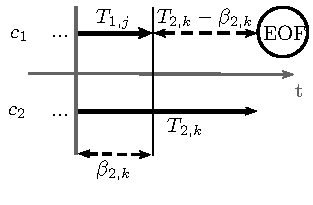
\includegraphics[width=\linewidth]{Figures/scheduler-case-2.pdf}}
        \end{center}
        \end{minipage}
        \caption{\label{fig:scheduler-cases} The $\beta$ value and illustrated Scheduler Cases 1 (b) and 2 (c): Both cases are close to the end of the file, meaning $c_1$ and $c_2$ can download the remaining bytes in their next requests while staying within their upper request limits $T_{1,max}$ and $T_{2,max}$.}
  \vspace*{-0.3cm}
\end{figure*}

Let $T_{i,j}$ be the time to transmit the $j$-th chunk over $c_i$; we have
\begin{equation}
\label{eq:time}
T_{i,j} = s_{i,j} / \overline{R}_i,
\end{equation}
In order to simplify our algorithm design, we assume that $\overline{R}_i$ does not change during the transmission of the $j$-th chunk, while $T_{i,j}$ is calculated. 

As discussed before in~\xref{sec:core-problem}, \mhttp~introduces a delay each time it performs a range 
request over a connection. This delay equals half of the latency of the connection, \ie the 
time that it takes for the HTTP range request to reach the server. Hence, the 
effective throughput $E_i$ of $c_i$, during the transmission of the $j$-th chunk, can be 
estimated as 
$$E_i = \frac{s_{i,j}}{T_{i,j} + 0.5 \overline{rtl}_i}$$
Let $T_{i,j} = \alpha_{i,j} \cdot \overline{rtl}_i$. Using \equref{eq:time}, we have
$$E_i=\frac{\alpha_{i,j} \cdot \overline{R}_i}{\frac{1}{2} + \alpha_{i,j}}.$$ 
$\alpha_{i,j}$ should be sufficiently large so that the effective throughput is larger than a certain 
threshold. In particular, with $\alpha_{i,j}=20$ we can ensure that $E_i > 0.975 \cdot \overline{R}_i$. 
Therefore, we set $T_{i,max}=20 \cdot \overline{rtl}_{i}$ as the maximum value for $T_{i,j}$ . 
In the other term, using our algorithm, we do not request chunks larger than 
$s_{i,max}=20 \cdot \overline{R}_i \cdot \overline{rtl}_{i}$, as requesting larger chunks does not bring
a significant gain. 

In order to avoid the connection idle times towards the end of the download, a special attention needs to be paid when assigning the size of the last chunks over each path to guarantee that the downloads of these last chunks complete at {\it roughly} the same time. 

Let $L$ be the size of the file and $\delta$ the amount of data that has been already 
downloaded/requested. Further, let $\beta_{i,j}$ be the time between the $j$-th scheduling 
decision for $c_i$ and the estimated time until the other connection completes its current 
download (see~\fref{fig:scheduler-cases} (a)).\footnote{$\beta_{i,j}$ is set to infinity if $c_i$ is the only 
established connection.} 
We consider four cases when determining the size of the next chunk 
over $c_i$. We specify the value of $T_{i,j}$ in each of these cases (note that $s_{i,j} = \overline{R}_i \cdot T_{i,j}$). 
Without loss of generality, we focus on the case where the scheduler wants to determine the next chunk for $c_2$. 

\begin{itemize}
\item Case 1 (\fref{fig:scheduler-cases}(b)): $c_2$ can download all remaining $L-\delta$ bytes  
within a time less than $T_{2,max}$ and before the other connection completes its current chunk download, 
\ie $\overline{R}_2 \cdot \beta_{2,j} \geq L-\delta$ and $ \overline{R}_2 \cdot T_{2,max} \geq L-\delta$. In this case, $T_{2,j}$ is the 
time required to download $L-\delta$, \ie $T_{2,j} = \frac{L-\delta}{\overline{R}_2}$.

\item Case 2 (\fref{fig:scheduler-cases} (b)): $\overline{R}_2 \cdot \beta_{2,j} < L-\delta$, but there exists a $T_{2,j} \leq T_{2,max}$ such that  
%but none of them can download $L-\delta$ in a single request. 
%In this case $T_{1,j}$ is the time in which $c_1$ is likely to finish with $c_2$'s upcoming time slice $T_{1,j} - \beta_{1,j}$:
%In the other term, there exists a $T_{i,j} \leq T_$ 
$$T_{2,j} \cdot \overline{R}_2 + (T_{2,j} - \beta_{2,j}) \cdot \overline{R}_1 = L-\delta.$$
In this case, the scheduler sets 
\begin{equation}
\label{eq:case2}
T_{2,j} = \frac{L-\delta + \beta_{2,j}\cdot \overline{R}_1}{\overline{R}_1 + \overline{R}_2}
\end{equation}
to guarantee that $c_1$ and $c_2$ complete their last chunk download at the same time.

\item Case 3: $\frac{L-\delta + \beta_{2,j}\cdot \overline{R}_1}{\overline{R}_1 + \overline{R}_2} > T_{2,max}$, 
hence, at least three more chunks will need to be fetched over $c_1$ and 
$c_2$ to download the remaining $L-\delta$ bytes. In this case, the maximum 
allowed time span is assigned in order to keep the request overhead low, \ie
$$T_{2,j} = T_{2,max}$$

\item Case 4: $c_2$ is a newly established connection ($j=1$). 
As the scheduler is not aware of the quality of the connection, it 
performs a range request for a relatively small chunk in order to probe the path quality. 
We denote by $initial$ the maximum size of the initial chunk that is allowed 
to be transmitted over a newly established connection; then $s_{2,1}=\min\{initial, L-\delta\}$. 
The value of $initial$ is an input to our scheduler. 
\end{itemize}
Algorithm~\ref{alg:advanced-scheduling} summarizes our scheduler design.

%This reduces the chunk size scheduling problem to only determining an optimal time span $T_{i,j}$.

%We define $\beta_{i,j}$ as the time span between the $j$th scheduling decision of path $i$ and the closest estimated time until another connection finishes downloading its current chunk, as depicted in figure \ref{fig:scheduler-cases} (a). 
%Further we need to determine the maximum allowed time span $T_{i,max}$ for a chunk scheduled over connection $i$, in order to establish an upper limit for a scheduled time slice: 

%$$T_{i,max} = \alpha \cdot rtt_i$$

%where our experiments showed that $\alpha$ should be a value between 20 and 30. 
%This is derived from calculations of the effective throughput $E_i$ of a connection $c_i$. 
%It is the throughput that takes into account the overhead of chunking the data, thus sending more requests and it is defined as the number of transmitted bytes during $\alpha \cdot rtt_i$ divided by the total transmission time on connection $c_i$, $\Omega_i$:

%$$E_i = \frac{\alpha \cdot rtt_i \cdot R_i}{\Omega_i}$$

%where the total transmission time $\Omega_i$ can be calculated through:

%$$\Omega_i = \alpha \cdot rtt_i + 0.5\cdot rtt_i$$

%Putting both equation together we get for the effective throughput:

%$$E_i = \frac{\alpha \cdot R_i}{\frac{1}{2} + \alpha}$$

%When trying to achieve an effective throughput $E_i$ of $\gamma$\% of the physical throughput $R_i$, we can calculate: 

%$$\frac{\alpha \cdot R_i}{\frac{1}{2} + \alpha} = \gamma \cdot R_i $$
%$$\Rightarrow \alpha = \frac{1}{2(\frac{1}{\gamma} - 1)}$$

%Lets say $E_i$ should be at least 95\% of $R_i$, we can calculate that $\alpha$ has to be at least 9.5 to achieve that goal.

%Given a file size $L$, an already downloaded amount of bytes $\delta$ from that file and a round-trip-time estimate $rtt_i$ for a connection $c_i$, when determining the optimal download time span $T_{i,j}$ we distinguish between three cases: \newline 
%\begin{itemize}
%\item Case 1 as depicted in \ref{fig:scheduler-cases}: The connection $c_1$ could download all remaining bytes $L-\delta$ within its upper limit $T_{1,max}$ and before $c_2$ finishes downloading its chunk. 
%In this case $T_{1,j}$ is the time necessary for $c_1$ to download $L-\delta$:

%$$T_{1,j} = \frac{L-\delta}{R_1}$$

%\item Case 2 as depicted in \ref{fig:scheduler-cases}: $c_1$ and $c_2$ could download $L-\delta$ within their next requests while staying inside their upper limits $T_{1,max}$ and $T_{2,max}$ respectively, but none of them could download $L-\delta$ in a single request.
%In this case $T_{1,j}$ is the time in which $c_1$ is likely to finish with $c_2$'s upcoming time slice $T_{1,j} - \beta_{1,j}$:

%$$T_{1,j} \cdot R_1 + (T_{1,j} - \beta_{1,j}) \cdot R_2 = L-\delta$$
%$$\Rightarrow T_{1,j} = \frac{L-\delta + \beta_{1,j}\cdot R_2}{R_1 + R_2}$$

%\item Case 3 describes cases in which $c_1$ and $c_2$ would need at least 3 more requests together to download $L-\delta$ while staying within their upper limits $T_{1,max}$ and $T_{2,max}$.

%In this case we simply assign the maximum allowed time span, to keep the request overhead low:

%$$T_{1,j} = T_{1,max}$$
%\end{itemize}

%For two active paths $c_i$ and $c_j, j \neq i$, the algorithm to determine a time slice $T_{1,j}$ then works as follows:

%\begin{algorithm}
%\caption{Synchronized Chunk Scheduling.}
%\label{alg:advanced-scheduling}
%\begin{algorithmic}
%\STATE{Init: $END \gets FALSE$}
%\STATE{$CONSTRAINT \gets (\beta_{i,j} \cdot R_i \geq L-\delta$ \OR $(END$ \AND $R_i > 0.9\cdot R_k))$}
%\IF{$T_{i,max} \cdot R_i \geq L-\delta$ \AND $CONSTRAINT$}
%        \STATE{$T_{i,j} \gets \frac{L-\delta}{R_i}$}
%\ELSE
%        \STATE{$T_{i,j} \gets \frac{L-\delta + \beta_{i,j} \cdot R_k}{R_i + R_k}$}
%        \IF{$T_{i,j} \leq T_{i,max}$}
%                \STATE{$END \gets TRUE$}
%        \ELSE
%                \STATE{$T_{i,j} \gets T_{i,max}$}
%        \ENDIF
%\ENDIF
%\end{algorithmic}
%\end{algorithm}

\begin{algorithm}
\caption{\algslice~Algorithm}
\label{alg:advanced-scheduling}
\begin{algorithmic}
\STATE{Init: $END \gets FALSE$}
\STATE{$CONSTRAINT \gets (\beta_{i,j} \cdot \overline{R}_i \geq L-\delta$ \OR ($END$ \AND $\overline{R}_i > 0.9\cdot \overline{R}_k))$}
\IF{$j=1$}
	\STATE{$s_{i,1}\gets \min\{initial, L-\delta\}$}
\ELSE
\IF{$T_{i,max} \cdot \overline{R}_i \geq L-\delta$ \AND $CONSTRAINT$}
	\STATE{$T_{i,j} \gets \frac{L-\delta}{\overline{R}_i}$}
\ELSE
	\STATE{$T_{i,j} \gets \frac{L-\delta + \beta_{i,j} \cdot \overline{R}_k}{\overline{R}_i + \overline{R}_k}$}
	\IF{$T_{i,j} \leq T_{i,max}$}
		\STATE{$END \gets TRUE$}
	\ELSE
		\STATE{$T_{i,j} \gets T_{i,max}$}
	\ENDIF
\ENDIF
\ENDIF
\end{algorithmic}
\end{algorithm}

The \term{END} Flag is important to be able to enter the first case and finish the download. 
We observe that with this algorithm the chunk size gets smaller towards the end of the file, which results in $\beta$ becoming smaller too, which means that without the \term{END} Flag the algorithm would tend to get stuck in the second case with very small chunk sizes. 
Further the \term{CONSTRAINT} Flag ensures that the last chunk in case 1 will be preferably downloaded by a connection with relatively good throughput.

In~\fref{fig:scheduler-flows} (b) we can see an illustrative example of how the chunk sizes evolve with this scheduler on a $4$MB file download. 
The measurements were conducted in our controlled German testbed described in~\xref{sec:evaluation-testbed}.
We observe that the scheduler tends to request relatively large chunks in the middle of the download. 
Towards the end the chunks become smaller. 
This example shows how the scheduler tries to avoid request overhead in the middle of the download, while trying to synchronize the chunk downloads towards the end of the file. 
Note, that this behavior also tends to lead to a higher request overhead towards the end of the file. 

%\begin{figure}[htbp]
%	\centering
%		\includegraphics[width=\linewidth]{Figures/flow-graph-synch.pdf}
%		\rule{35em}{0.5pt}
%	\caption[Flow Graph]{An illustrative example of how the chunk sizes evolve in case of a $4$MB file download.}
%	\label{fig:flow_graph_synch}
%\end{figure}
